\chapter{Análisis}

\section{Arquitectura}
El objetivo del chatbot es conseguir información estructurada a partir de las experiencias y emociones de los usuarios. Con este objetivo se ha desarrollado un proyecto que consta de dos componentes principales: una aplicación web y un chatbot en Telegram. La aplicación web actúa como panel de control para que el administrador tenga acceso a la gestión de preguntas, así como consultar las respuestas de los usuarios. 

Para asegurar la eficacia, se hace uso de una base de datos tipo PostgreSQL que almacena tanto las preguntas como las repsuestas lo que permite un fácil acceso a esta información. Gracias a esto se consigue una solución integral que combina la facilidad de uso del chatbot en Telegram con la capacidad de gestión y análisis dada por la aplicación web. \vspace{7cm}


\begin{figure}[!ht]
    \centering
    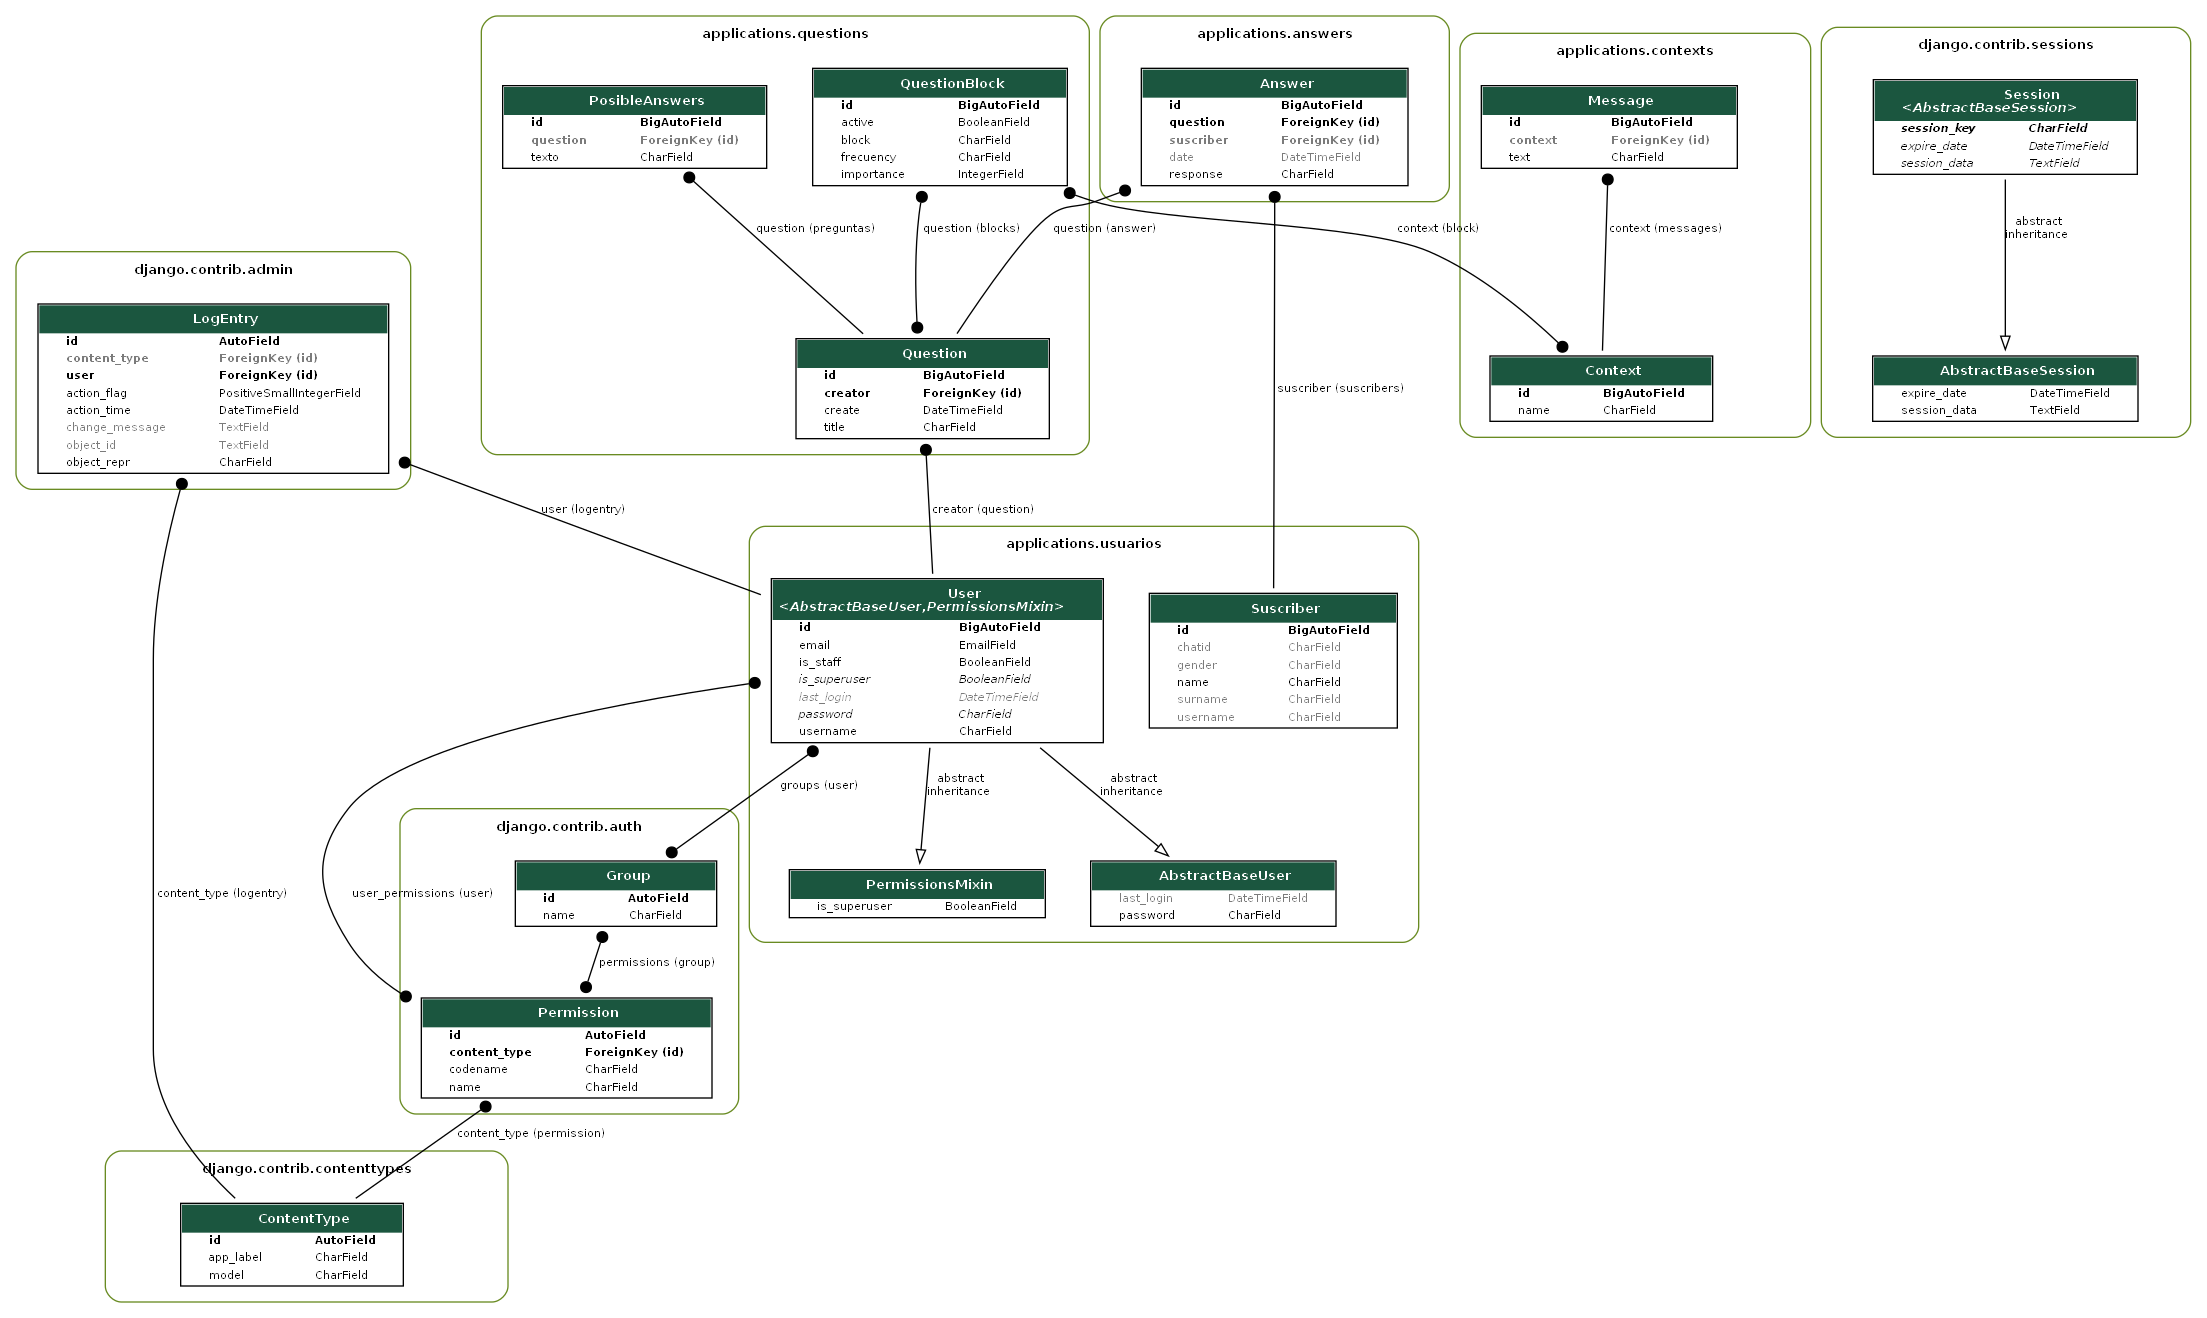
\includegraphics[width=1\textwidth, height=15cm]{imagenes/myapp_models.png}
    \caption{ Diagrama de clases }
    \label{fig:enter-label}
\end{figure}


Esta base de datos consta de cinco entidades principales:
\begin{itemize}
\item \textbf{Peguntas}: Contiene la información de todas las preguntas almacenadas. Esta se divide en dos: Pregunta y Posibles respuestas. Dentro de la primera especificaría el título de la pregunta junto con otros campos como la fecha o usuario de creación y la segunda contiene las respuestas a esa pregunta. 
\item \textbf{Bloques de Preguntas}: Las preguntas se almacenan en bloques. Cada bloque puede tener las preguntas que desee, además de un atributo booleano que indicará que ese bloque de preguntas se encuentra activo. Los bloques también tienen asociado un contexto. 
\item \textbf{Contextos}: Dentro de los contextos se guardan los mensajes a mostrar por el bot cuando se hable de un tema concreto. Si un bloque tiene asociado un contexto, en el momento que se realice el cuestionario asociado a ese bloque de preguntas el bot mostrará cualquiera de los mensajes de ese contexto de forma aleatoria. De esta forma nos aseguramos la interactividad y que la experiencia sea diferente para cada usuario.
\item \textbf{Usuarios}: Guarda los agentes registrados en nuestro sistema. Se divide en dos tipos: los administradores que tienen acceso al panel de control y los usuarios comúnes que son los que interactúan con el bot.
\item \textbf{Respuestas}: Contiene las respuestas de los usuarios a las preguntas. Solo se almacenan las respuestas posibles de cada pregunta para así confirmar que la información sea correcta.
\end{itemize}

La parte del chatbot está formada por tres módulos. Un primer módulo de bienvenida y registro, donde el bot se presenta con el usuario y lo registra en nuestra base de datos. Un segundo módulo que actúa como agente conversacional y un tercer módulo que representa el cuestionario de preguntas. Posteriormente los analizaremos con más detalle.

Esta arquitectura permite creación de cuestionarios interactivos, almacenamiento de datos y análisis de respuestas de forma confidencial para su posterior evaluación.

\begin{figure}[h]
    \centering
    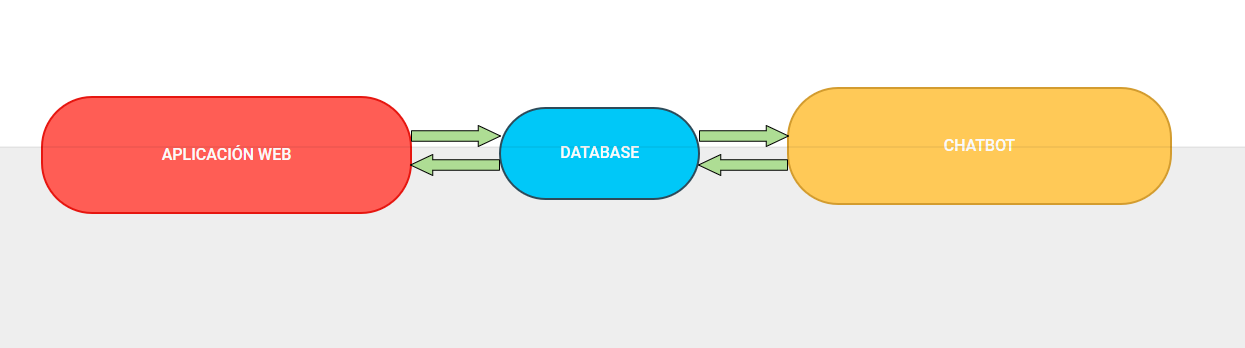
\includegraphics[width=1\textwidth]{imagenes/arquitecture.png}
    \caption{\textit{POSTCOVID-AI TELEGRAMBOT} arquitectura}
    \label{fig:enter-label}
\end{figure}

\section{Implementación}
Para el desarrollo usaremos herramientas de Front-End, que nos ayudarán a dar cuerpo a nuestro sitio web y herramientas de Back-End para el control y lógica tanto de la web como del bot. Las tecnologías utilizadas para la implementación del proyecto son las siguientes:

\begin{itemize}
\item \textit{\textbf{Python}} como lenguaje principal del bot y de la web.
\item \textit{\textbf{Django}} es un framework de aplicaciones web gratuito y de código abierto (open source) escrito en Python para el desarrollo de nuestra web.
\item \textit{\textbf{Telegram}} como plataforma para alojar el chatbot
\item \textit{\textbf{Python-telegram-bot}} es una librería de Python para la creación de nuestro bot que nos permite conectarnos a la API de Telegram.
\item \textit{\textbf{PostgreSQL}} es un sistema de gestión de base de datos relacional orientado a objetos.
\item \textit{\textbf{Psycopg2}} para adaptar la base de datos a Python.
\item \textit{\textbf{HTML5}} lenguaje para la elaboración de páginas web.
\item \textit{\textbf{CSS3}} como lenguaje de diseño gráfico para crear la presentación de nuestra página.
\item \textit{\textbf{Javascript}} para dar dinamismo a nuestra web y ayudar en la experiencia del usuario.
\item \textit{\textbf{Foundation}} como framework de ayuda a la hora de crear la interfaz de usuario.
\item \textit{\textbf{Docker}} para automatizar el despliegue de la aplicación dentro de un contenedor software.
\item \textit{\textbf{Github}} como tecnología que nos ayuda a realizar copias del proyecto y controlar versiones.
\end{itemize}


\section{Funcionamiento}
Antes de empezar con el desarrollo de nuestro proyecto, debemos definir la funcionalidad del mismo explicando detalladamente como sería el comportamiento de cada una de las partes implicadas.

\begin{itemize}
\item \textbf{Web}: Creación de una interfaz con la que poder interaccionar con las preguntas del bot y mensajes a mostar.
\begin{itemize}
\item Implementación de un login y un registro para que solo los usuarios registrados puedan acceder al panel de control.
\item Panel de control, primera vista del usuario que funciona como guía para las operaciones a realizar.
\item Apartado de preguntas, bloques, contextos, preguntas e información y gestión de usuarios.
\item Vistas de detalle y operaciones de modificación y borrado de cada uno de los apartados anteriores.
\item Autenticación y permisos en la realización de operaciones solo para usuarios específicos.
\item Descarga de las respuestas proporcionadas por los usuarios en formato CSV.

\end{itemize}
\item \textbf{Chatbot}: Creación de un chatbot en línea que realice un cuestionario de preguntas y a su vez una lógica interna que permita una interacción con el usuario.
\begin{itemize}
\item Mensaje de bienvenida al usuario cuando entre en el chat del bot.
\item Almacenamiento del usuario como un nuevo integrante de nuestro sistema si ningún tipo de cuestionario gracias a las funciones especificas de Telegram que permiten la obtención de los datos del usuario que se encuentra activo en el chat.
\item Entorno de interacción por parte del bot con el usuario para poder tener una conversación lo más humana posible mediante el análisis de ciertas palabras e ideas previamente establecidas.
\item Cuestionario de preguntas que se encuentran activas para cada usuario en un momento concreto. Estas preguntas varían dependiendo de los bloques que el administrador tenga activos y la frecuencia de cada uno de ellos.
\item Recolección y almacenamiento de las respuestas proporcionadas en la base de datos de forma automática.
\item Lógica para identificar cada vez que el usuario cuente con preguntas activas.
\item Creación de un aviso diario al usuario cuando haya preguntas sin responder.
\end{itemize}
\end{itemize}
